\begin{table}[h]
\centering
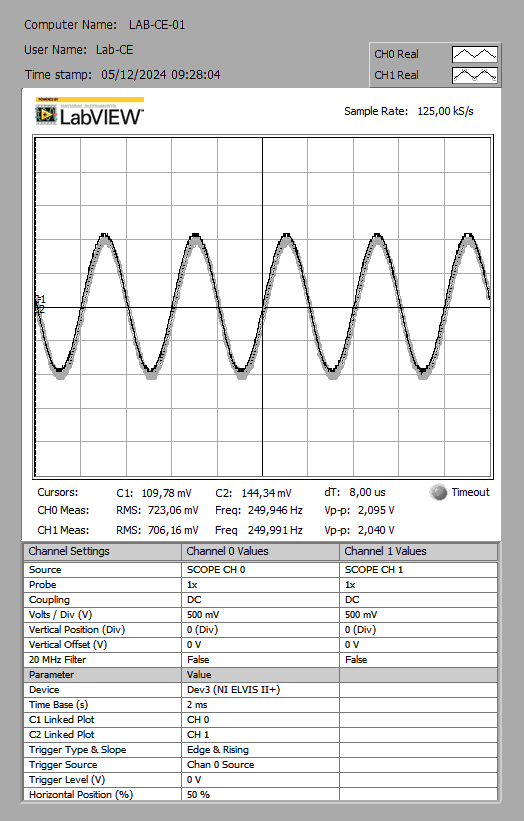
\includegraphics[scale=0.725]{rgadicoas/rgadicoa1}
\end{table}

\begin{center}
Gráfico 9: Tensão da fonte e $V_1$ em $f=250Hz$
\end{center}

\begin{table}[h]
\centering
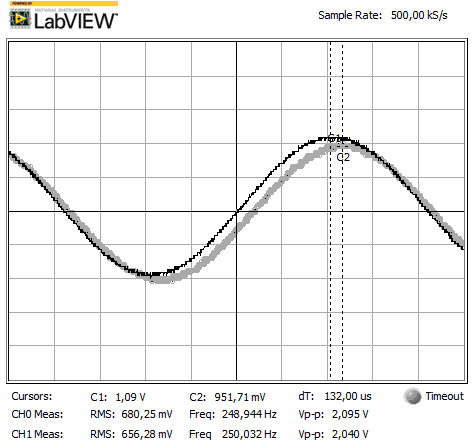
\includegraphics[scale=0.725]{rgadicoas/rgadicoa1-2}
\end{table}

\begin{center}
Gráfico 10: Tensão da fonte e $V_1$ em $f=250Hz$ (ampliado)
\end{center}

Amplitude $V_1$: $1,02V$, dt: $136\mu s\implies$ Fase $V_1$: $-12,26$\textdegree 

\newpage
\begin{table}[h]
\centering
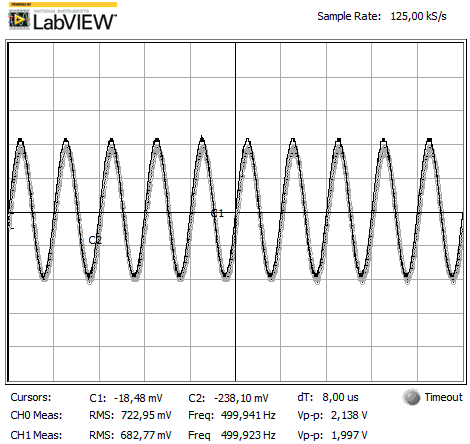
\includegraphics[scale=0.725]{rgadicoas/rgadicoa2}
\end{table}

\begin{center}
Gráfico 11: Tensão da fonte e $V_1$ em $f=500Hz$ 
\end{center}

\begin{table}[h]
\centering
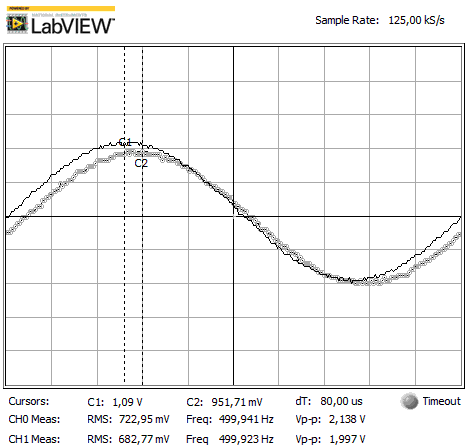
\includegraphics[scale=0.725]{rgadicoas/rgadicoa2-2}
\end{table}

\begin{center}
Gráfico 12: Tensão da fonte e $V_1$ em $f=500Hz$ (ampliado)
\end{center}

Amplitude $V_1$: $0,999V$, dt: $80\mu s\implies$ Fase $V_1$: $-14,38$\textdegree

\newpage
\begin{table}[h]
\centering
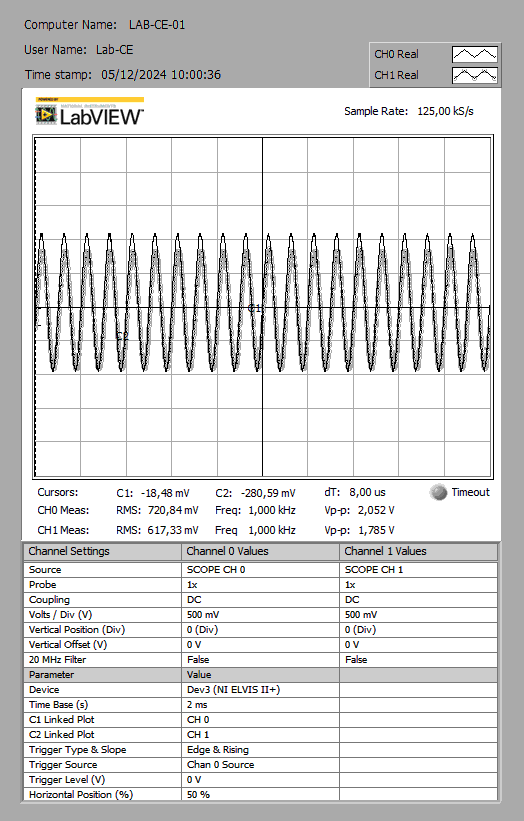
\includegraphics[scale=0.725]{rgadicoas/rgadicoa3}
\end{table}

\begin{center}
Gráfico 13: Tensão da fonte e $V_1$ em $f=1000Hz$ 
\end{center}

\begin{table}[h]
\centering
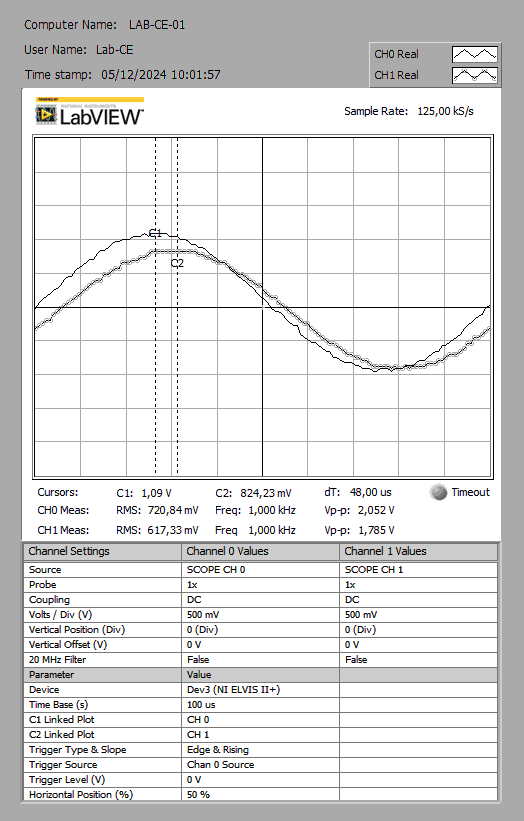
\includegraphics[scale=0.725]{rgadicoas/rgadicoa3-2}
\end{table}

\begin{center}
Gráfico 14: Tensão da fonte e $V_1$ em $f=1000Hz$ (ampliado)
\end{center}

Amplitude $V_1$: $0,893V$, dt: $48\mu s\implies$ Fase $V_1$: $-17,30$\textdegree

\newpage
\begin{table}[h]
\centering
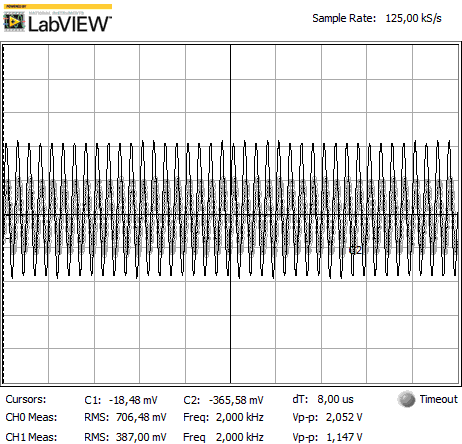
\includegraphics[scale=0.725]{rgadicoas/rgadicoa4}
\end{table}

\begin{center}
Gráfico 15: Tensão da fonte e $V_1$ em $f=2000Hz$ 
\end{center}

\begin{table}[h]
\centering
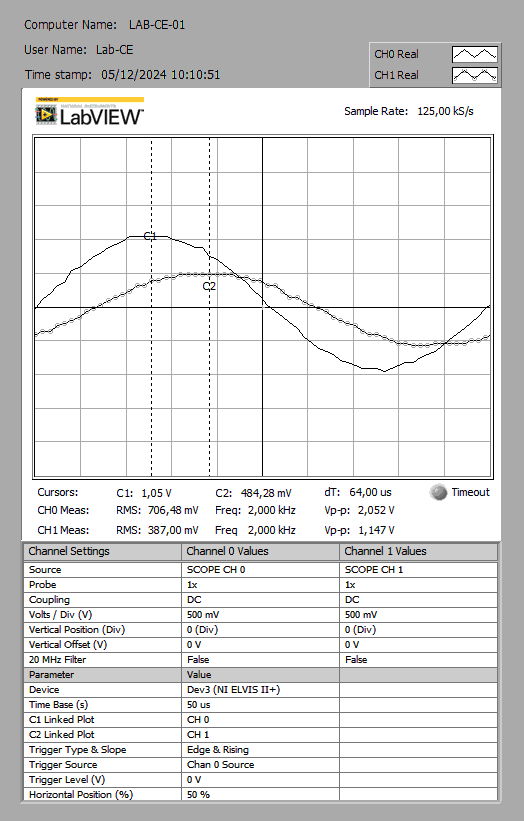
\includegraphics[scale=0.725]{rgadicoas/rgadicoa4-2}
\end{table}

\begin{center}
Gráfico 16: Tensão da fonte e $V_1$ em $f=2000Hz$ (ampliado)
\end{center}

Amplitude $V_1$: $0,574V$, dt: $64\mu s\implies$ Fase $V_1$: $-46,07$\textdegree

\newpage
\begin{table}[h]
\centering
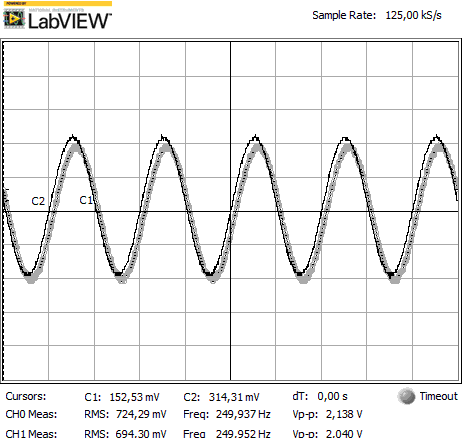
\includegraphics[scale=0.725]{rgadicoas/rgadicoa5}
\end{table}

\begin{center}
Gráfico 17: Tensão da fonte e $V_2$ em $f=250Hz$ 
\end{center}

\begin{table}[h]
\centering
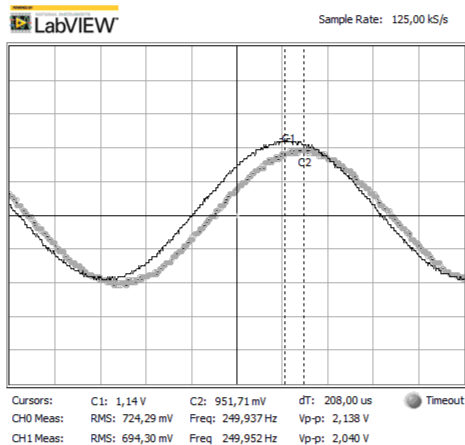
\includegraphics[scale=0.725]{rgadicoas/rgadicoa5-2}
\end{table}

\begin{center}
Gráfico 18: Tensão da fonte e $V_2$ em $f=250Hz$ (ampliado)
\end{center}

Amplitude $V_2$: $1,02V$, dt: $208\mu s\implies$ Fase $V_2$: $-18,74$\textdegree

\newpage
\begin{table}[h]
\centering
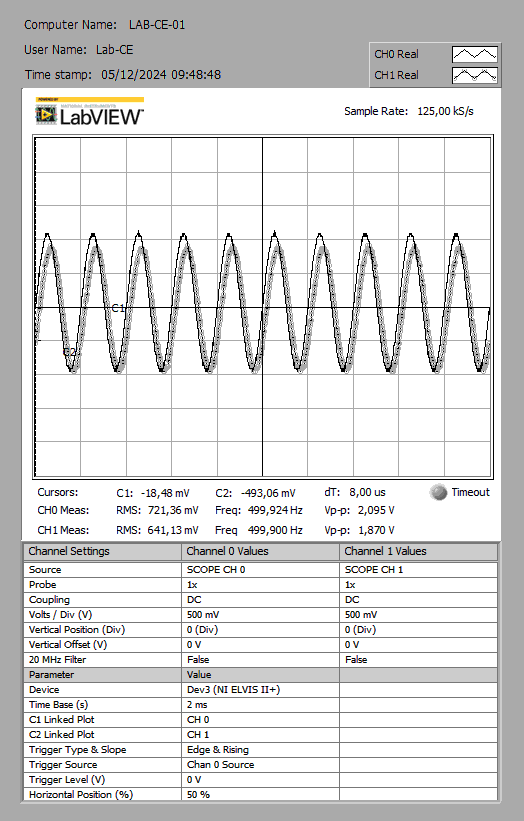
\includegraphics[scale=0.725]{rgadicoas/rgadicoa6}
\end{table}

\begin{center}
Gráfico 19: Tensão da fonte e $V_2$ em $f=500Hz$ 
\end{center}

\begin{table}[h]
\centering
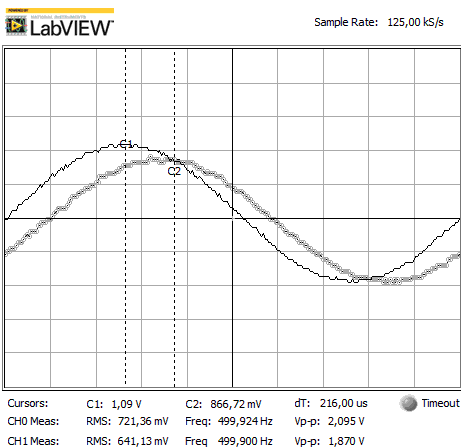
\includegraphics[scale=0.725]{rgadicoas/rgadicoa6-2}
\end{table}

\begin{center}
Gráfico 20: Tensão da fonte e $V_2$ em $f=500Hz$ (ampliado)
\end{center}

Amplitude $V_2$: $0,935V$, dt: $216\mu s\implies$ Fase $V_2$: $-38,90$\textdegree

\newpage
\begin{table}[h]
\centering
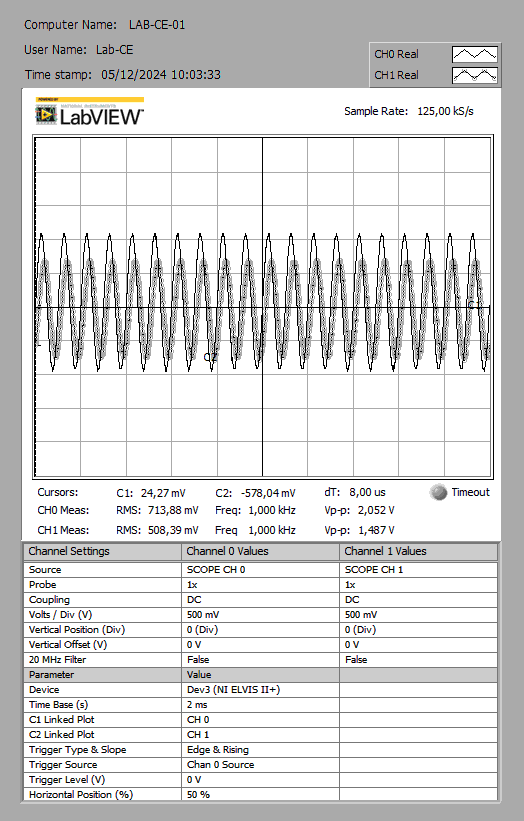
\includegraphics[scale=0.725]{rgadicoas/rgadicoa7}
\end{table}

\begin{center}
Gráfico 21: Tensão da fonte e $V_2$ em $f=1000Hz$ 
\end{center}

\begin{table}[h]
\centering
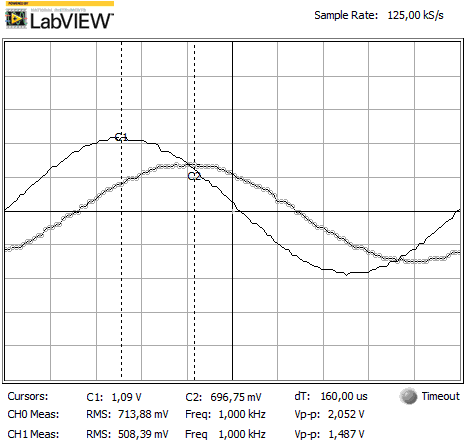
\includegraphics[scale=0.725]{rgadicoas/rgadicoa7-2}
\end{table}

\begin{center}
Gráfico 22: Tensão da fonte e $V_2$ em $f=1000Hz$ (ampliado)
\end{center}

Amplitude $V_2$: $0,744V$, dt: $160\mu s\implies$ Fase $V_2$: $-57,58$\textdegree

\newpage
\begin{table}[h]
\centering
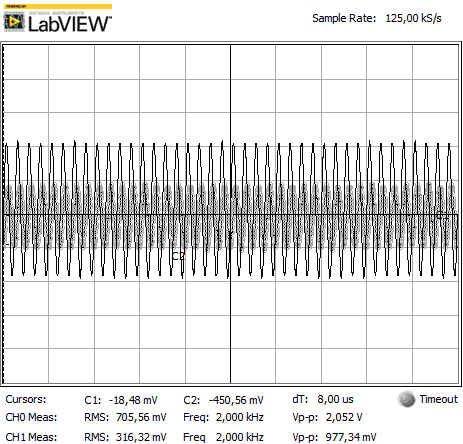
\includegraphics[scale=0.725]{rgadicoas/rgadicoa8}
\end{table}

\begin{center}
Gráfico 23: Tensão da fonte e $V_2$ em $f=2000Hz$ 
\end{center}

\begin{table}[h]
\centering
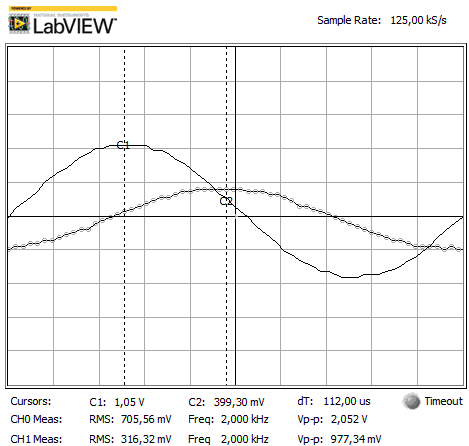
\includegraphics[scale=0.725]{rgadicoas/rgadicoa8-2}
\end{table}

\begin{center}
Gráfico 24: Tensão da fonte e $V_2$ em $f=2000Hz$ (ampliado)
\end{center}

Amplitude $V_2$: $0,489V$, dt: $112\mu s\implies$ Fase $V_2$: $-80,62$\textdegree